\section{Matrices: array of numbers}

%Lecture 9.11




Matrices are rectangular arrays of numbers:

$$
A = 
\left[
\begin{matrix}
a_{11} & a_{12} & ... & a_{1n} \\
a_{21} & a_{22} & ... & a_{2n} \\
... & ... & ... & ...\\
a_{m1} & a_{m2} & ... & a_{mn}
\end{matrix}
\right] \in \Re^{m\times n}
$$


The element in the $i^{th}$ row \& $j^{th}$ column: $a_{ij} = [A]_{ij}$(equivalent notation)

The transposition operation works on matrices by exchanging rows and columns: 

$$
A^T = 
\left[
\begin{matrix}
a_{11} & a_{21} & ... & a_{1n} \\
a_{12} & a_{22} & ... & a_{m2} \\
... & ... & ... & ...\\
a_{1n} & a_{2n} & ... & a_{mn}
\end{matrix}
\right] \in \Re^{m\times n}
$$

So $[A]_{ij}  = [A^T]_{ji}$ if $A\in \Re^{m\times n}$ and $A^T\in \Re^{n\times m}$


1) $A + B = C$ where $[C] = [A]_{ij} + [B]_{ij}$

2) $\alpha A = B$ where $[B]l_{ij} = \alpha [A]_{ij}$

The origin is a all-zero matrix. 

\begin{definition}{Inner Product}
	$<A, B> = trace(A^TB) = trace(BA^T)$ where $A^TB\in \Re^{n\times n}$ and $B^TA\in \Re^{m\times m}$
\end{definition}

where trace(X) is defined as the sum of the diagonal elements of X. \\

Forbenius Norm: $||A||_F = \sqrt{<A, A>} = \sqrt{trace(A^TA)} = \sqrt{\sum^m_{i=1}\sum^m_{j=1}[A]^2_{ij}}$


$$\vec{(A)} = \text{vec}
\left(
\left[
\begin{matrix}
... & ... & ... & ... \\
a_{1} & a_{2} & ... & a_{n} \\
... & ... & ... & ...
\end{matrix}
\right]\right) = 
\left[
\begin{matrix}
a_{1} \\
a_{2} \\
... \\
a_{n}
\end{matrix}
\right]
\in \Re^{m\times n}
$$

Matrix inverse: if $A$ is "invertible", $\exists$ unique $A^{-1}$ s.t. $AA^{-1} = A^{-1}A = I$

\begin{itemize}
	\item $(AB)^{-1} = B^{-1}A^{-1}$
	
	\item $(A^{-1})^T = (A^T)^{-1}$
	
	\item $det(A^{-1}) = \frac{1}{det(A)}$
\end{itemize}

\subsection{Matrices as linear \& affine maps}


$x\in \Re^n \rightarrow A \rightarrow y = Ax \in \Re^m$\\

Affine maps are linear functions plus a constant term: $y = Ax + b$ where $A\in \Re^{m,n}$, $b\in \Re^m$

\subsection{Approximations}

A nonlinear map $f: \Re^n \rightarrow \Re^m$ can be approximated by an affine map:

\begin{equation*}
f(x) = f(x_0) + J_f(x_0)(x - x_0) + o(||x - x_0||)
\end{equation*}

where $o(||x - x_0||)$ are terms go to 0 faster than 1st order for $x\rightarrow x_0$ and $J_f(x_0)$ is the Jacobian of $f$ at $x_0$:




$$J_f(x_0) = 
\left[
\begin{matrix}
\frac{\sigma f_1}{\sigma x_1} &  ... & \frac{\sigma f_1}{\sigma x_n} \\
... &  ... & ...\\
\frac{\sigma f_m}{\sigma x_1} &  ... &\frac{\sigma f_m}{\sigma x_n}
\end{matrix}
\right]_{x = x_0}
$$

For $x$ 'near' $x_0$, the variation $\delta_f(x) =f(x) - f(x_0)$ can be approximated described by a linear map:

\begin{equation*}
\delta_f(x) = J_f(x_0)\delta_x, \,\, \delta_x = x - x_0
\end{equation*}
\subsection{Orthogonal Matrices}

\begin{definition}
	$U\in \Re^{n\times m}$ is \textbf{orthogonal} if $U = [U^{(1)} ... U^{(n)}]$
	and 
	
	$$ U^{(1)^T}U^{(1)}=\left\{
	\begin{aligned}
	0\,\, \forall i\neq j \\
	1\,\, if \,\, i = j
	\end{aligned}
	\right.
	$$
\end{definition}

Then $UU^T = U^TU = I$\\


$x\rightarrow U \rightarrow y = Ux$

\begin{equation*}
||y||^2 = (Ux)^T(Ux) = x^TU^TUx = x^Tx = ||x||^2
\end{equation*}

$<Ux, Uw> = x^TU^TUw = x^Tw = <x, w>$

\begin{itemize}
	\item Domain
\end{itemize}

$dom(A)$ = $\Re^n$, $A = [a^{(1)}...a^{(n)}]$

$dom(A^T)$ = $\Re^m$, $A^T = [a^{(1)}...a^{(m)}]$


\begin{itemize}
	\item Range
\end{itemize}

Range of A is the set of vectors $y$ obtained as a linear combination of the $a_i$s are of the form $y= Ax$ for some vector $x\in \Re^n$.

\begin{equation*}
R(A) = \{y\in \Re^m | y = Ax = \sum^n_{i=1}x_ia^{(i)}\}
\end{equation*}

\begin{equation*}
R(A^T) = \{w\in \Re^m | w = A^Tu = \sum^m_{i=1}u_ia^{(i)}\}
\end{equation*}

\begin{itemize}
	\item Rank
\end{itemize}

The dimension of $R(A)$ is called the rank of $A$:

\begin{equation*}
rank(A) = dim\{R(A)\} = dim\{R(A^T)\} = rank(A^T)
\end{equation*}

\begin{itemize}
	\item Nullspace
\end{itemize}

The nullspace of the matrix $A$ is he set of vectors in the input space that are mapped to zero:

\begin{equation*}
N(A) = \{x\in \Re^n | Ax = 0\}
\end{equation*}

\begin{itemize}
	\item Fundamental Theorem
\end{itemize}

We can find that for any $x\in \Re(A^T)$ and any $z\in \mathcal{N}(A)$, it holds that $x^Tz = 0$.\\

$\Re^n = \Re(A^T) \bigoplus N(A)$: $\forall x\in \Re^n$ there is a unique $x = x_{R(A^T)} = x_{N(A)}$.\\

\begin{theorem}{Fundamental theorem of linear algebra}
	For any given matrix $A\in \Re^{m,n}$, it holds that $\mathcal{N}(A) \perp \mathcal{R}(A^T)$ and $\mathcal{R}(A) \perp \mathcal{N}(A^T)$, hence
	
	\begin{align*}
	\mathcal{N}(A) \bigoplus \mathcal{R}(A^T) &= \Re^n\\
	\mathcal{R}(A) \bigoplus \mathcal{N}(A^T) &= \Re^m\\
	dim \mathcal{N}(A) + rank(A) &=n\\
	dim \mathcal{N}(A^T) + rank(A) &=m
	\end{align*}
\end{theorem}

Consequently we can decompose $\forall x\in \Re^n$ as the sum of 2 vectors orthogonal to each other, one in range of $A^T$ and another in nullspace of $A$:

\begin{equation*}
x = A^T\xi + z, z\in \mathcal{N}(A)
\end{equation*}




\subsection{PageRank}

%Lecture Sep 16

For the PageRank algorithm, more important webpages should be ranked higher:


Let us assume each node’s importance score is evenly spread across all the outgoing links, each node’s importance score can also be written as the sum of the importance scores received from all of the incoming neighbors: for node A, $\sum_{j \rightarrow A}\frac{\pi_j}{O_j}$


\begin{figure}
	\centering
	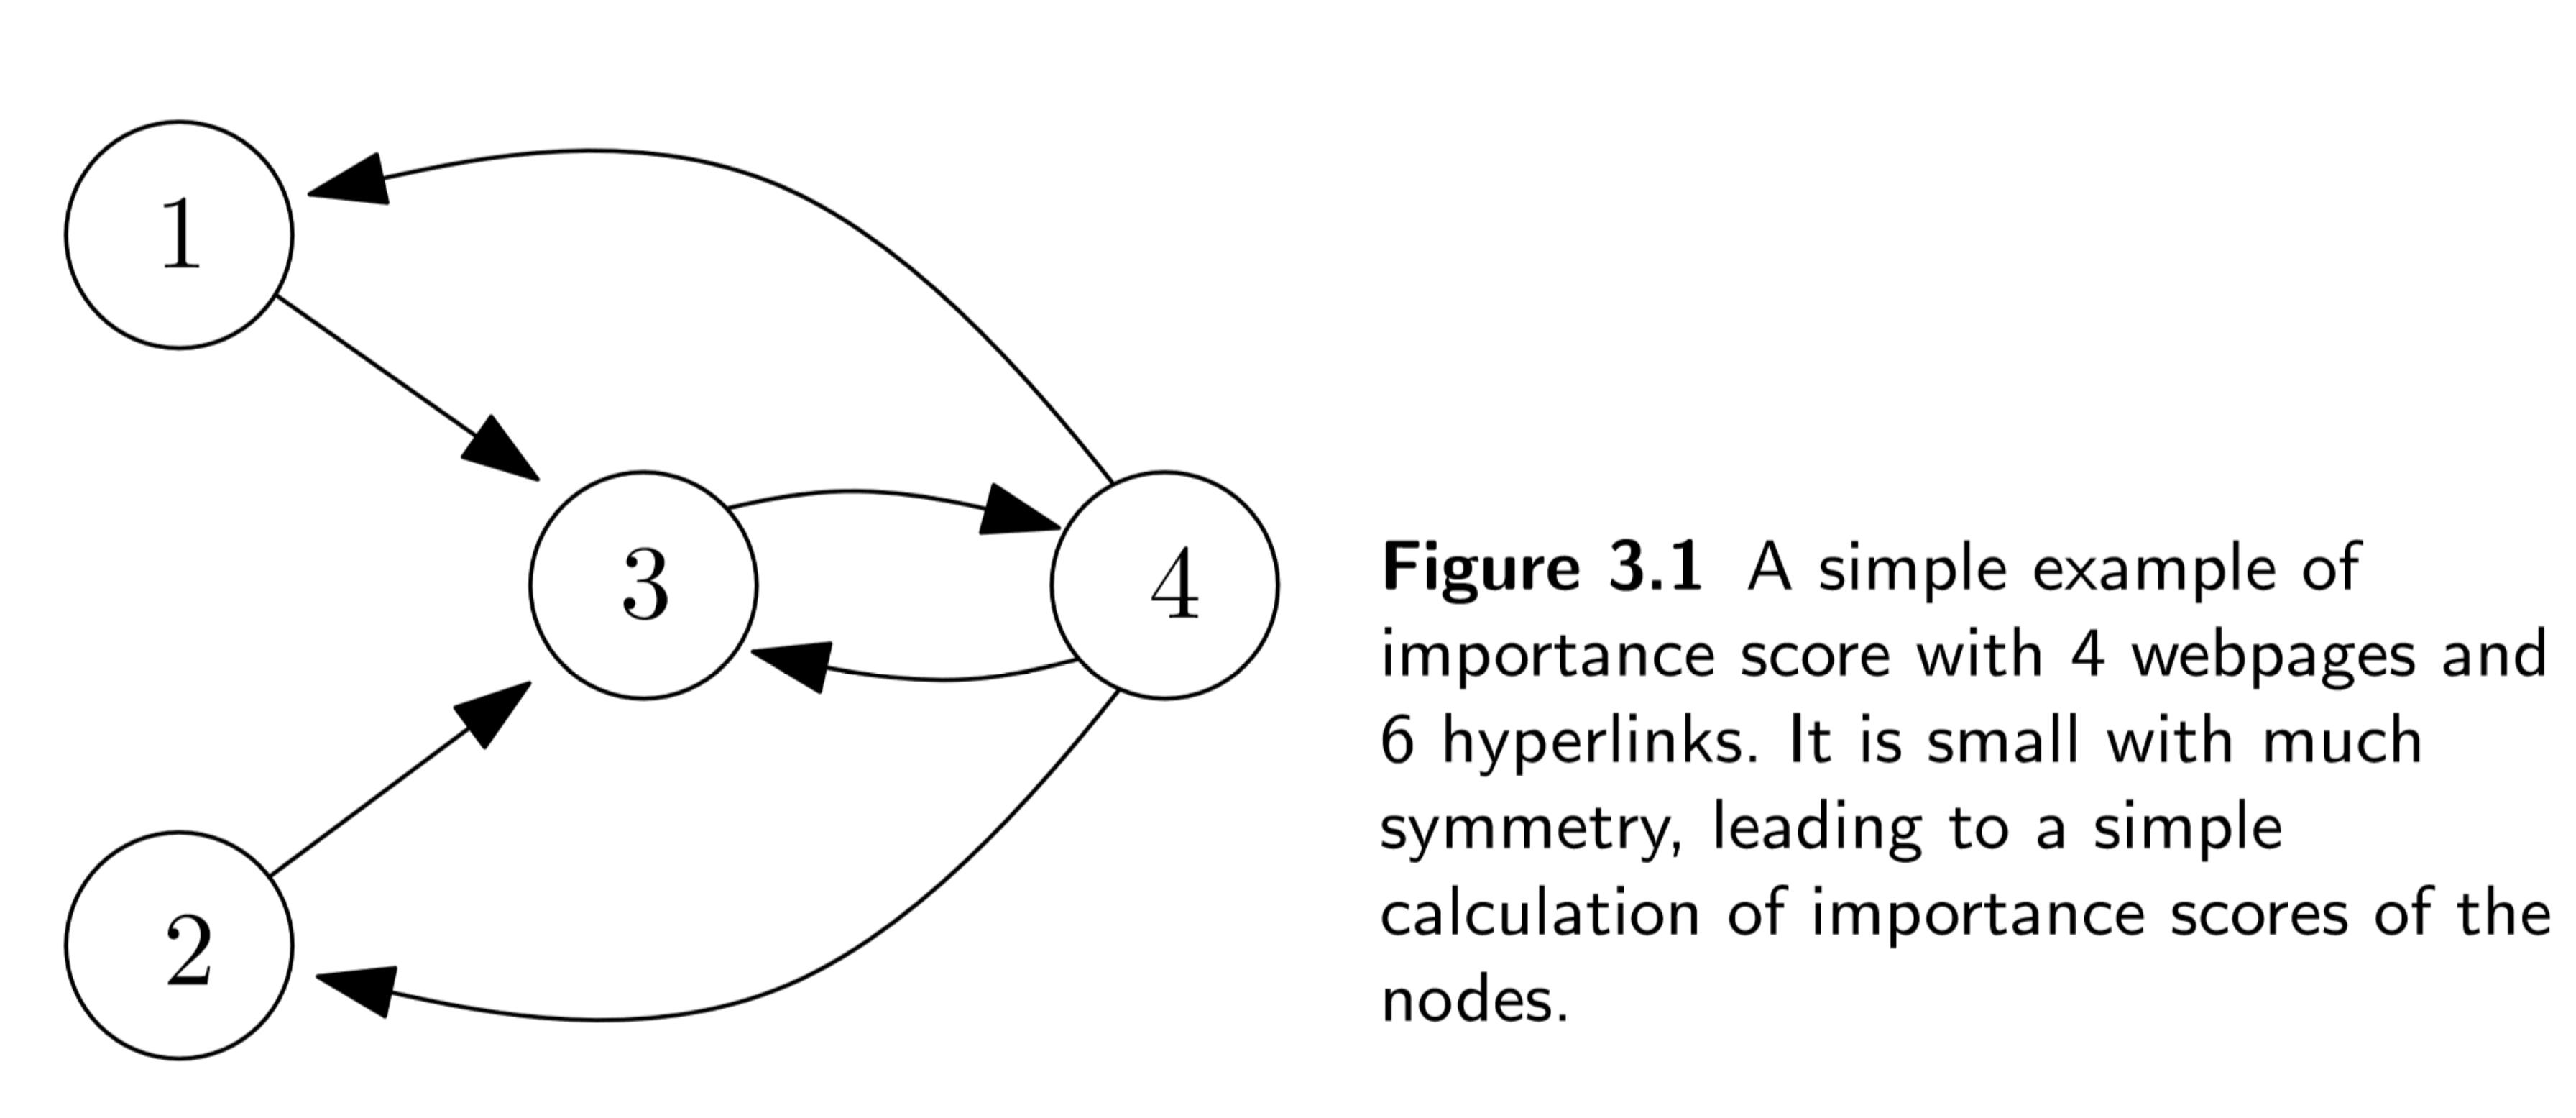
\includegraphics[width=2.1in,height=2.1in]{figures/ch03/figure0.jpg}
	%\caption{This is an inserted JPG graphic} 
	%\label{fig:graph} 
\end{figure}


Let the score of node 1 (and 2) be x, and that of node 3 (and 4) be y. Looking at node 1's incoming links, we see that there is only one such link, coming from node 4 that points to three nodes. So $x = \frac{y}{3}$ and $2x + 2y = 1$, so set of importance scores turns out to be [0.125, 0.125, 0.375, 0.375].

Matrix $H$: its $(i,j)$th entry is $\frac{1}{O_i}$ if there is a hyperlink from webpage i to webpage j, and 0 otherwise.

$\pi$: $N \times$1 column vector denoting the importance scores of the N webpages.

Multiply $\pi^T$ on the right by matrix $H$, this is spreading the importance score from the last iteration evenly among the outgoing links, and re-calculating the importance score of each webpage in this iteration by summing up the importance scores from the incoming links.

Note: $\pi^T[k] = \pi^T[k - 1]H$



Note: $\pi^T[k] = \pi^T[k - 1]G$

Obviously, $\pi^{T}$ is the left eigenvector of $G$ corresponding to the eigenvalue of 1: $\pi^{T} = \pi^{*T}G$.

For a graph like this:

\begin{figure}
	\centering
	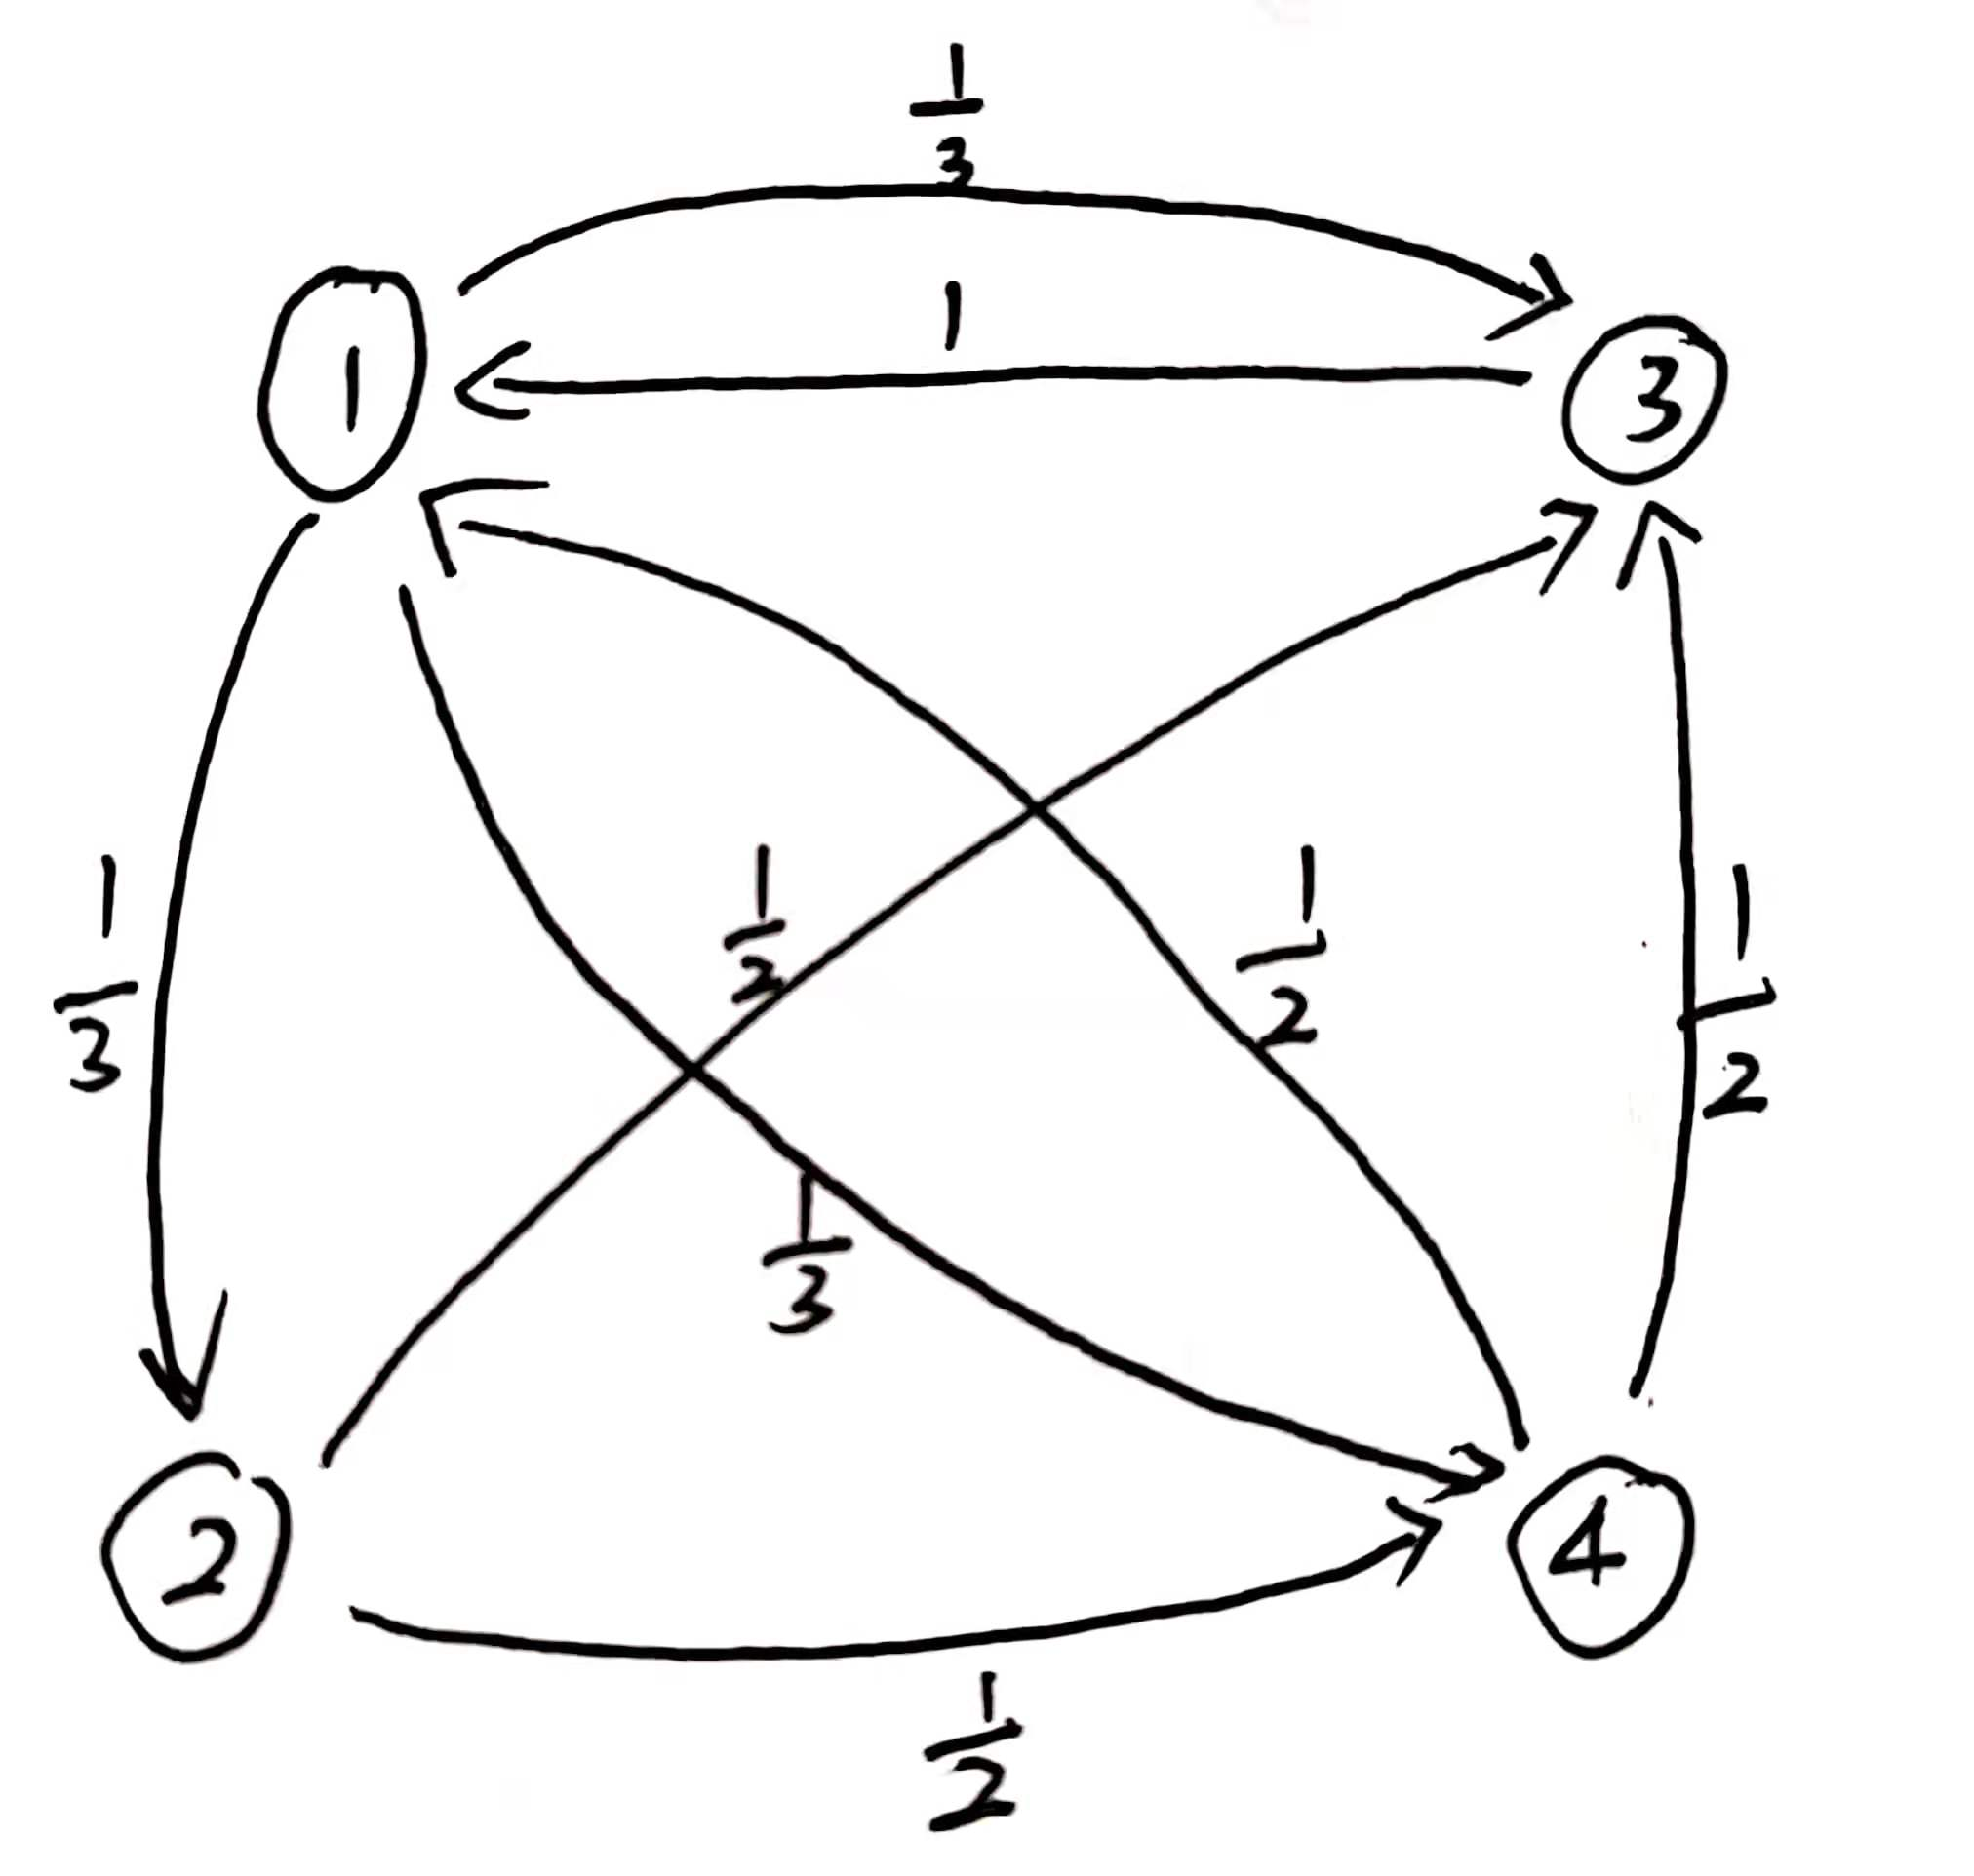
\includegraphics[width=2.1in,height=2.1in]{figures/ch03/figure3.jpg}
	%\caption{This is an inserted JPG graphic} 
	%\label{fig:graph} 
\end{figure}



$$
\left[
\begin{matrix}
x_1 \\
x_2 \\
x_3\\
x_4\\
\end{matrix}
\right] =
\left[
\begin{matrix}
0 & 0 & 1 & \frac{1}{2} \\
\frac{1}{3} & 0 & 0& 0 \\
\frac{1}{3}& \frac{1}{2} & 0 & \frac{1}{2} \\
\frac{1}{3} & \frac{1}{2} & 0 & 0 
\end{matrix}
\right]
\left[
\begin{matrix}
x_1 \\
x_2 \\
x_3\\
x_4\\
\end{matrix}
\right]
$$

\begin{align*}
x &= Ax \\
Ax - x &= 0\\
(A - I)x &= 0\\
x&\in N(A-I)
\end{align*}


$$
x = \frac{1}{s_1}
\left[
\begin{matrix}
12 \\
4 \\
9\\
6\\
\end{matrix}
\right]
$$
Note: 

\begin{itemize}
	\item $x^{(0)}$ is the initial distribution.
	
	\item $x^{(0)}_i = $Pr[start on page $i$]
	
	\item $u^{(i)}, \lambda_i$ is eigen-vector/value pair if $Au^{(i)} = \lambda_iu^{(i)}$
\end{itemize}


If $Au^{(i)} = \lambda_iu^{(i)}$, $A$ is "diagonalizable" if it has a full set of linear independent eigenvectors. In this case $x^{(0)} = \sum^n_{i=1}\alpha_iu^{(i)}$

\begin{align*}
x^{(1)} &= Ax^{(0)} = A[\sum^n_{i=1}\alpha_iu^{(1)} = \sum_i\alpha_i(Au^{(i)})]\\
x^{(2)} &= A(Ax^{(0)}) = \sum^n_{i=1}\alpha_i(A^2u^{(i)}) = \sum^n_{i=1}\alpha_i(\lambda_i^2u^{(i)})\\
...\\
x^{(k)} &= A^kx{(0)} = \sum^n_{i=1}\alpha_i(\lambda_i)^ku^{(i)}\\
&= \alpha_1(\lambda_1)^ku^{(1)} + \sum^n_{i=2}\alpha_i(\lambda_i)^ku^{(i)} \\
&= \alpha_1u^{(1)} + \sum^n_{i=2}\alpha_i(\lambda_i)^ku^{(i)}\\
&when \,k \rightarrow \infty\\
&= \alpha_1u^{(1)}
\end{align*}

\begin{equation*}
lim_{k\rightarrow \infty}\frac{A^kx^{(0)}}{||A^kx^{(0)}||} =u^{(i)}
\end{equation*}

%What is an Internet Structure s.t. $dim[N(A-I)] = 2$?

If have repeated eigenvalues:

\begin{align*}
Au^{(1)} =\lambda_1u^{(1)}\\
Au^{(2)} =\lambda_2u^{(2)}
\end{align*}

clearly:

\begin{equation*}
A(\alpha_1u^{(1)} + \alpha_2u^{(2)}) = \alpha_1\lambda_1u^{(1)} + \alpha_2\lambda_2u^{(2)}
\end{equation*}

where $\alpha_1u^{(1)} + \alpha_2u^{(2)}$ is this linear combination and $\alpha_1\lambda_1u^{(1)} + \alpha_2\lambda_2u^{(2)}$ are the maps to a different of same eigenvalues.

1) The "algebraic" multiplicity of an eignevalue $\lambda$ of a square matrix $A$ is \# of eigenvalues $\lambda_i, \lambda_2,...,\lambda_m$ equal to $\lambda$. $\rightarrow$ AM($\lambda$)

2) The geometric multiplicity of an eigenvalue $\lambda$ of a square matrix $A$ is the dimension of $N(A - \lambda I)$. $\rightarrow$ GM($\lambda$)

In general, $0 < GM(\lambda) \leq AM(\lambda)$ \& If $GM(\lambda_i) = AM(\lambda_i)$, $\forall i$, then $A$ is diagonalizable. 


If diagonalizable, we can write $Au^{(i)} = \lambda_iu^{(i)} \rightarrow$ assume all $\lambda_i$ distinct $GM(\lambda_i) = AM(\lambda_i) = 1, \forall i$

$$
\left[
\begin{matrix}
Au^{(1)} & Au^{(2)} &... &Au^{(n)} 
\end{matrix}
\right] =
\left[
\begin{matrix}
\lambda_1u^{(1)} & \lambda_2u^{(2)}&... &\lambda_iu^{(i)}
\end{matrix}
\right]
$$

$$A
\left[
\begin{matrix}
u^{(1)} & u^{(2)} &... &u^{(n)} 
\end{matrix}
\right] =
\left[
\begin{matrix}
u^{(1)} & u^{(2)} &... &u^{(n)}
\end{matrix}
\right]
\left[
\begin{matrix}
\lambda_1 & 0 & ... & 0\\
0& \lambda_2  &  ... & 0\\
...  & ...  &   ...& \\
0    &  ... &  0 & \lambda_n
\end{matrix}
\right]
$$



\begin{align*}
AU &= U\Lambda\\
A &= U\Lambda U^{-1}\\
\Lambda &= U^{-1}AU
\end{align*}

Recall pagerank:

\begin{align*}
A^kx^{(0)} &= (U\Lambda U^{-1})^kx^{(0)}\\
&=U\Lambda^kU^{-1}x^{(0)} \\
&= U
\begin{bmatrix}
\lambda_1^k & 0 & ... & 0\\
0& \lambda_2^k  &  ... & 0\\
...  & ...  &   ...& \\
0    &  ... &  0 & \lambda_n^k
\end{bmatrix} U^{-1}x^{(0)}
\end{align*}

\subsection{Determinant}

In eigen-decomposition, we need to solve for $\lambda$ from $det(A - \lambda I) = 0$. 
If $det(A) = 0$ then $A$ is non-invertible. 

Example:

$$A = 
\left[
\begin{matrix}
a_{11} & a_{12}\\
a_{21} & a_{22}
\end{matrix}
\right] =
\left[
\begin{matrix}
a_{(1)} & a_{(2)}
\end{matrix}
\right]
$$

\begin{align*}
U &= \{x\in \Re^2 | 0\leq x_1 \leq 1, 0\leq x_1 \leq 1 \}\\
P &= \{Ax, \ x\in \mathcal{U}\} 
\end{align*}

\begin{figure}
	\centering
	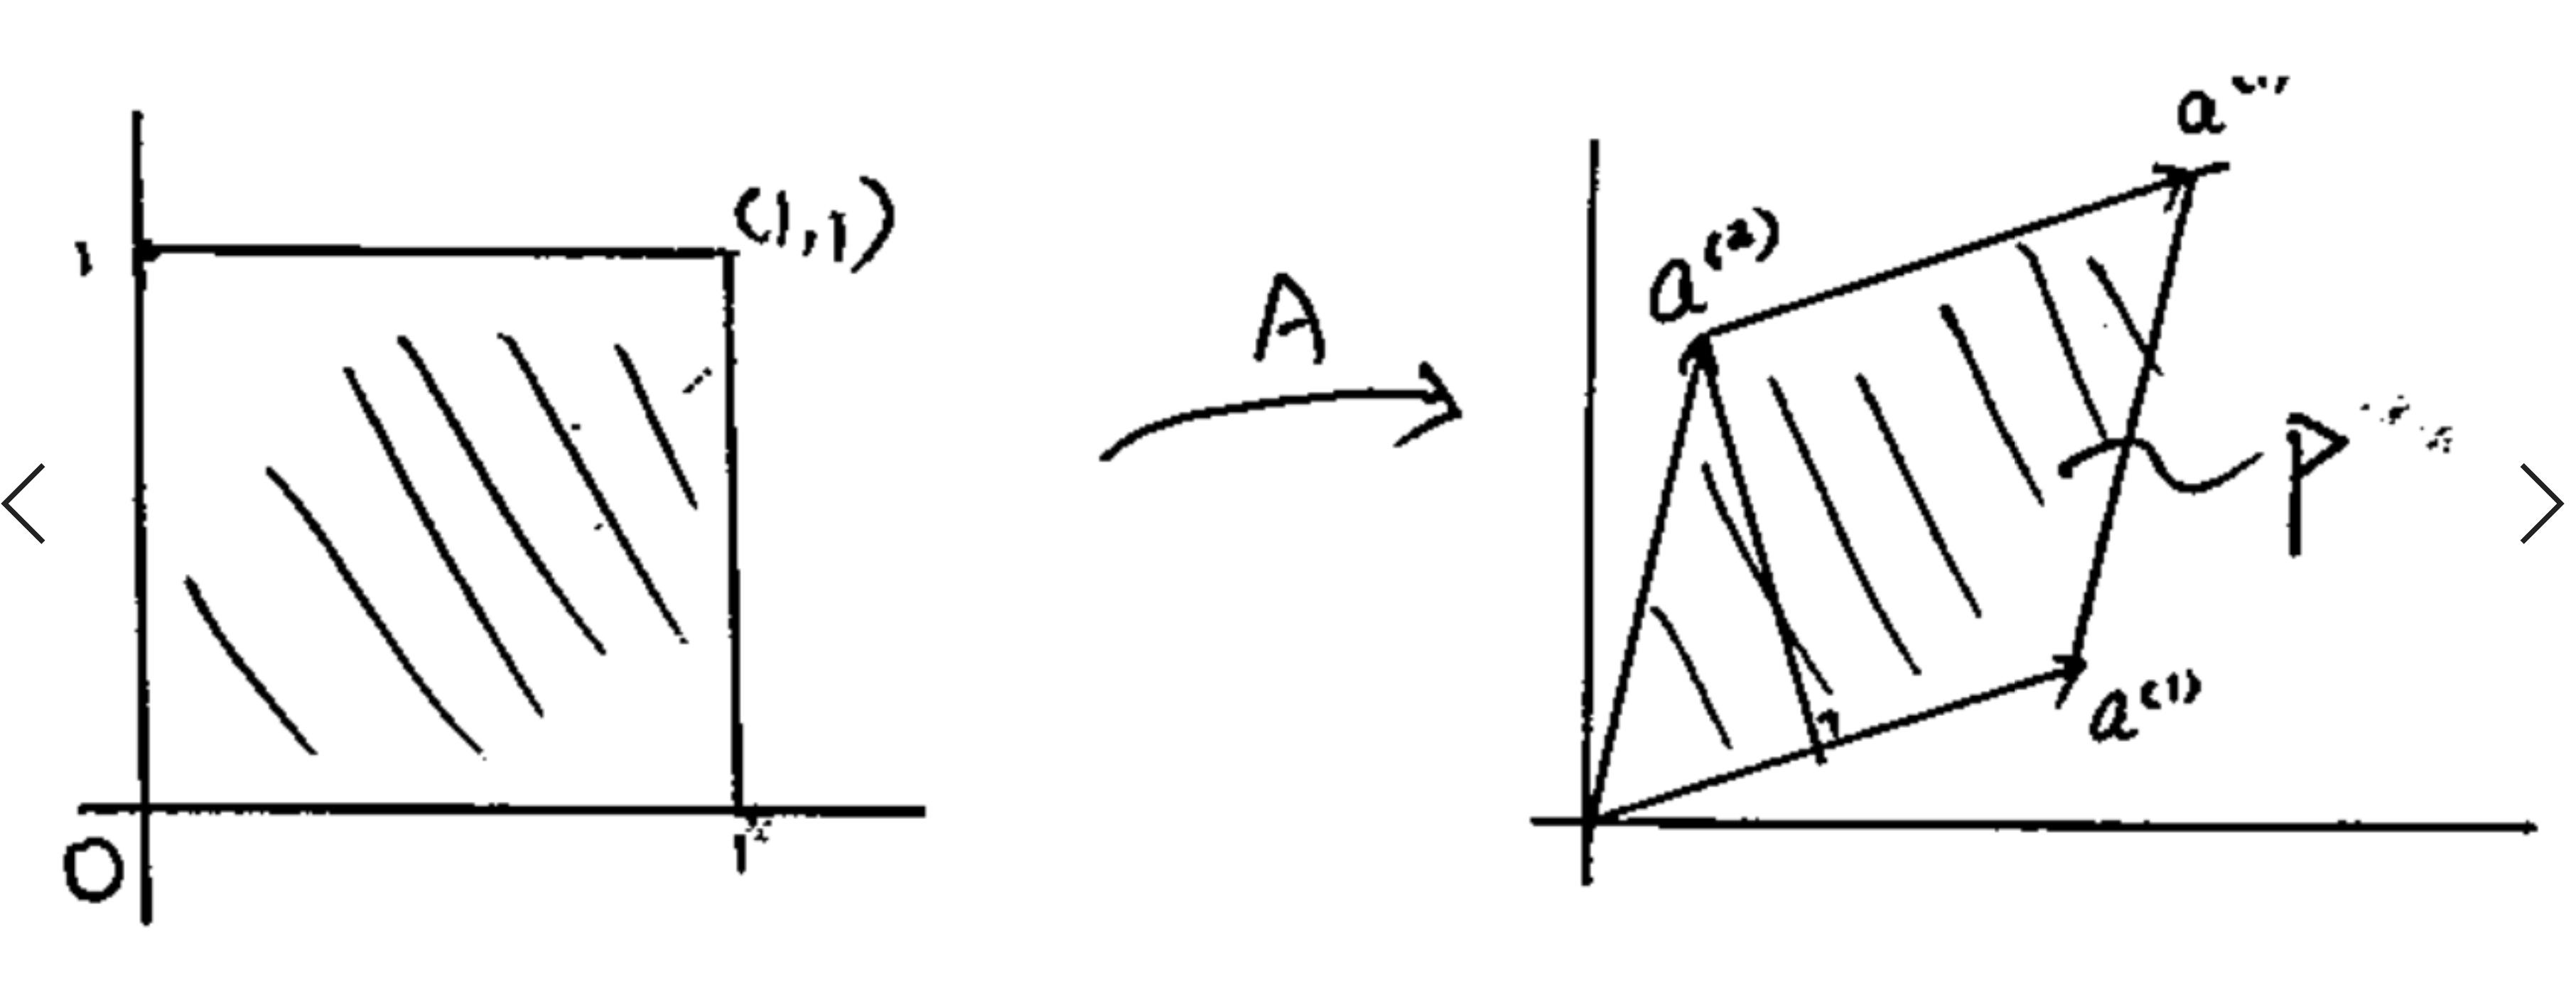
\includegraphics[width=2.1in,height=2.1in]{figures/ch03/figure1.jpg}
	%\caption{This is an inserted JPG graphic} 
	%\label{fig:graph} 
\end{figure}


Two matrices $A, B \in \Re^{n, n}$ are said to be \textbf{similar} if there exists a nonsingular matrix $P\in \Re^{n,n}$ s.t.:

\begin{equation*}
B = P^{-1}AP
\end{equation*}

Because there exists vectors $\tilde{x}, \tilde{y}$ s.t.:
\begin{align}
x &= P\tilde{x}\\
y &= P\tilde{y}\\
P\tilde{y} &= A P\tilde{x}\\
\tilde{y} &= P^{-1}AP P\tilde{x} = B \tilde{x}
\end{align}

Assume $A$ is \textbf{diagonalizable}(similar to a diagonal matrix):

\begin{align*}
A &= U\Lambda U^{-1}\\
|det(A)| &= |det(U\Lambda U^{-1})| \\
&= |det(U)det(\Lambda)det(U^{-1})|\\
&= det(U)det(\Lambda)\frac{1}{det(U)}\\
&= |det(\Lambda)|\\
&= |\prod^n_{i=1}\lambda_i|
\end{align*}

\begin{align*}
X: N(\mu, \Sigma)\,\,where\,\,(\mu \in \Re^n, \Sigma \in \Re^{n\times n})\\
P_x(x) = \frac{1}{(2\pi)^{\frac{2}{n}}}\frac{1}{|det\Sigma|^{\frac{1}{2}}}exp[-\frac{1}{2}(x - \mu)^T\Sigma^{-1}(x - \mu)]
\end{align*}
